\documentclass{article}
\usepackage[margin=0cm]{geometry}
\usepackage[utf8]{inputenc}
\usepackage{tikz}
\usepackage{graphicx,placeins}
\usepackage{enumitem}
\pagestyle{empty}
\usetikzlibrary{positioning, shapes.geometric, arrows, arrows.meta}



\usepackage[backend=biber,style=authoryear-comp,natbib=true]{biblatex}

\addbibresource{flowchart_bibliography.bib}


% TikZ styles
\tikzset{
    process/.style={
        rectangle, draw, rounded corners=5pt, inner sep=7pt,
        minimum width=9cm, minimum height=1.2cm,
        text width=9cm,
        font=\normalsize,
        align=center,
        fill=white, semithick
    },
    wideprocess/.style={
        rectangle, draw, rounded corners=5pt, inner sep=7pt,
        minimum width=8cm, minimum height=1.2cm,
        text width=7.7cm,
        font=\normalsize,
        fill=white, semithick
    },
    narrowprocess/.style={
        rectangle, draw, rounded corners=5pt, inner sep=7pt,
        minimum width=9cm, minimum height=2.75cm,
        text width=9.7cm,
        font=\normalsize,
        fill=white, semithick
    },
    decision/.style={
    diamond, draw, semithick, fill=white,
    aspect=2,                 % keeps diamond proportions
    minimum width=5.5cm,      % <-- fixed size for ALL decision nodes
    minimum height=2.2cm,
    text width=5.2cm,         % controls wrapping (adjust if needed)
    inner sep=0ex,            % consistent padding (avoid negative)
    align=center,
    font=\normalsize\bfseries
  },
    arrow/.style={-{triangle 45}, semithick}
}

% Global itemize spacing
\setlist[itemize]{leftmargin=*,label=\textbullet,topsep=0pt,itemsep=3pt,parsep=0pt}

\begin{document}

\begin{figure}[ht!]
    \centering
\resizebox{\textwidth}{!}{%
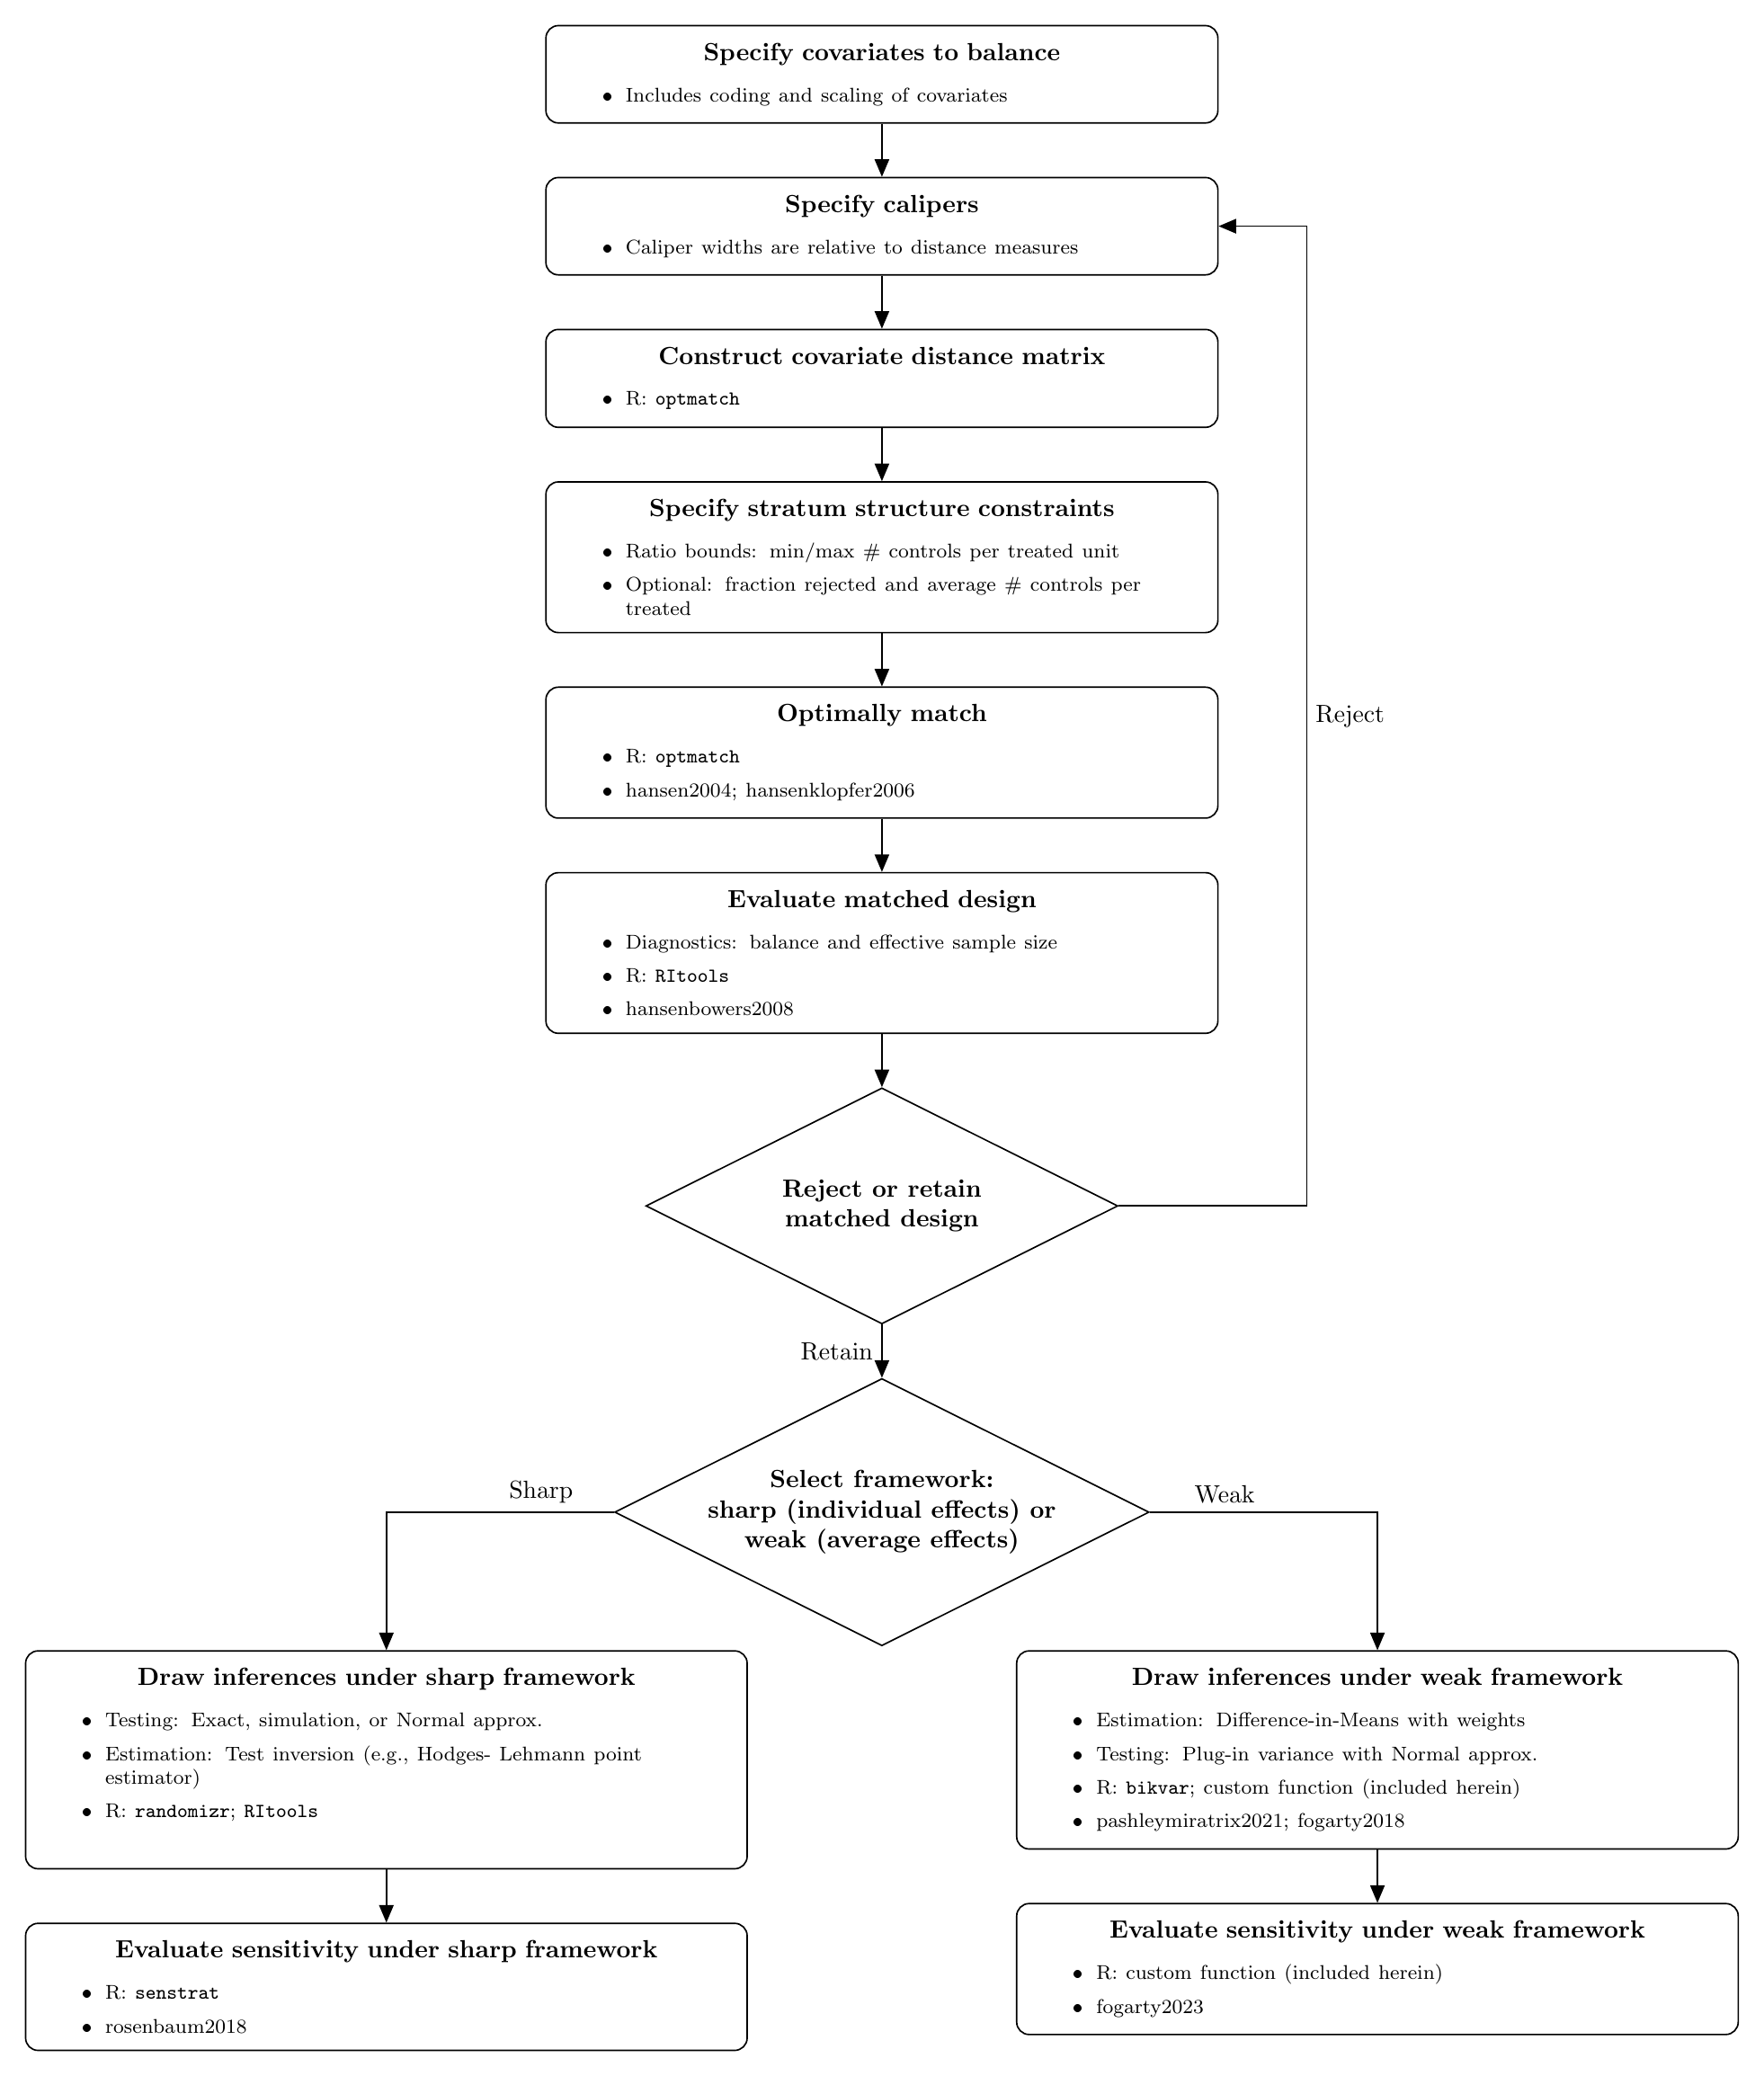
\begin{tikzpicture}[node distance=0.75cm, auto]

% Nodes
\node[process] (specify_covariates) {\centering\normalsize\textbf{Specify covariates to balance}\\[0.25cm]
    \raggedright\footnotesize
    \begin{itemize}
        \item Includes coding and scaling of covariates
    \end{itemize}
};

\node[process, below=of specify_covariates] (specify_calipers) {%
    \centering\normalsize\textbf{Specify calipers}\\[0.25cm]
    \raggedright\footnotesize
    \begin{itemize}
        \item Caliper widths are relative to distance measures
    \end{itemize}
};

\node[process, below=of specify_calipers] (construct_matrix) {%
    \centering\normalsize\textbf{Construct covariate distance matrix}\\[0.25cm]
    \raggedright\footnotesize
    \begin{itemize}
        \item R: \texttt{optmatch}
    \end{itemize}
};

\node[process, below=of construct_matrix] (specify_stratum) {%
    \centering\normalsize\textbf{Specify stratum structure constraints}\\[0.25cm]
    \raggedright\footnotesize
    \begin{itemize}
        \item Ratio bounds: min/max \# controls per treated unit
        \item Optional: fraction rejected and average \# controls per treated
    \end{itemize}
};

\node[process, below=of specify_stratum] (optimal_match) {%
    \centering\normalsize\textbf{Optimally match}\\[0.25cm]
    \raggedright\footnotesize
    \begin{itemize}
        \item R: \texttt{optmatch}
        \item \citet{hansen2004}; \citet{hansenklopfer2006}
    \end{itemize}
};

\node[process, below=of optimal_match] (evaluate_design) {%
    \centering\normalsize\textbf{Evaluate matched design}\\[0.25cm]
    \raggedright\footnotesize
    \begin{itemize}
        \item Diagnostics: balance and effective sample size
        \item R: \texttt{RItools}
        \item \citet{hansenbowers2008}
    \end{itemize}
};

\node[decision, below=of evaluate_design] (decision) {Reject or retain\\ matched design};

\node[decision, below=of decision] (target_selection) {Select framework:\\sharp (individual effects) or \\weak (average effects)};

\node[narrowprocess, below right=1cm and 0cm of target_selection] (weak_inference) {%
    \centering\normalsize\textbf{Draw inferences under weak framework}\\[0.25cm]
    \raggedright\footnotesize
    \begin{itemize}
        \item Estimation: Difference-in-Means with weights
        \item Testing: Plug-in variance with Normal approx.
        \item R: \texttt{bikvar}; custom function (included herein)
        \item \citet{pashleymiratrix2021}; \citet{fogarty2018}
    \end{itemize}
};

\node[narrowprocess, below left=1cm and 0cm of target_selection] (sharp_inference) {%
    \centering\normalsize\textbf{Draw inferences under sharp framework}\\[0.25cm]
    \raggedright\footnotesize
    \begin{itemize}
        \item Testing: Exact, simulation, or Normal approx.
        \item Estimation: Test inversion (e.g., Hodges- Lehmann point estimator)
        \item R: \texttt{randomizr}; \texttt{RItools}
        \item[] $ $ 
    \end{itemize}
};

\node[narrowprocess, below=of weak_inference, minimum height=1.2cm] (weak_sensitivity) {%
    \centering\normalsize\textbf{Evaluate sensitivity under weak framework}\\[0.25cm]
    \raggedright\footnotesize
    \begin{itemize}
        \item R: custom function (included herein)
        \item \citet{fogarty2023}
    \end{itemize}
};

\node[narrowprocess, below=of sharp_inference, minimum height=1.2cm] (sharp_sensitivity) {%
    \centering\normalsize\textbf{Evaluate sensitivity under sharp framework}\\[0.25cm]
    \raggedright\footnotesize
    \begin{itemize}
        \item R: \texttt{senstrat}
        \item \citet{rosenbaum2018}
    \end{itemize}
};

% Arrows
\draw[arrow] (specify_covariates) -- (specify_calipers);
\draw[arrow] (specify_calipers) -- (construct_matrix);
\draw[arrow] (construct_matrix) -- (specify_stratum);
\draw[arrow] (specify_stratum) -- (optimal_match);
\draw[arrow] (optimal_match) -- (evaluate_design);
\draw[arrow] (evaluate_design) -- (decision);

\draw[arrow] (decision) -- ++(6,0) |- node[near start, right] {Reject} (specify_calipers);
\draw[arrow] (decision) -- node[left] {Retain} (target_selection);
\draw[arrow] (target_selection) -| node[near start, above left] {Weak} (weak_inference);
\draw[arrow] (target_selection) -| node[near start, above right] {Sharp} (sharp_inference);
\draw[arrow] (weak_inference) -- (weak_sensitivity);
\draw[arrow] (sharp_inference) -- (sharp_sensitivity);

\end{tikzpicture}%
}

\caption{Flow diagram of the design-based matching pipeline}
%\label{fig:flowchart}
\end{figure}
\FloatBarrier

%\setlength{\bibitemsep}{0.5em}
%\printbibliography

\end{document}